\documentclass[11pt]{article}

% ---- arXiv-ready preamble: standard packages only ----
\usepackage[utf8]{inputenc}
\usepackage[T1]{fontenc}
\usepackage[margin=1in]{geometry}
\usepackage{times}
\usepackage{amsmath,amssymb}
\usepackage{graphicx}
\usepackage{booktabs}
\usepackage{array}
\usepackage{xcolor}
\usepackage{caption}
\usepackage[numbers,sort&compress]{natbib}
\usepackage{hyperref}
\hypersetup{colorlinks=true, linkcolor=blue!50!black, citecolor=blue!50!black,
            urlcolor=blue!50!black}
\usepackage{enumitem}

\newcommand{\impact}{\textsc{Impact}}
\newcommand{\bench}{PI-Bench}

\title{\bench: Can Agents Run a Research Lab?}
\author{Zhiwei Bao\\ Zhejiang University\\ \texttt{zwbao1996@zju.edu.cn}}
\date{}

\begin{document}
\maketitle

\begin{abstract}
Language-model agents are competent at short, well-specified tasks, but a research career
is not a task---it is a long chain of interdependent bets made under uncertainty, where
feedback is slow and the field keeps shifting. Real long-horizon agency demands a cluster
of capabilities that current benchmarks test in isolation, if at all:
(1)~inferring hidden state from noisy, biased signals;
(2)~making irreversible commitments that cannot be unwound;
(3)~planning under delayed, heavy-tailed rewards;
(4)~budgeting two scarce resources at once; and
(5)~exploring a non-stationary environment before it is obviously worth it.
\bench{} stresses these together by simulating one of the most information-poor,
delayed-reward jobs there is: running an academic lab for 60 months. The world is fully
mechanistic (no LLM judge in the reward path), partially observable, non-stationary, and
full of delayed, coupled consequences. Success is \impact{}---citations accrued plus a
projection of published work's future citations---a score built so that abandoning the
lab to hoard cash earns nothing. We evaluate twelve models spanning Alibaba Bailian and
OpenRouter; \impact{} spans more than an order of magnitude, every model captures only a
small fraction of the attainable citation ceiling, and---because a career turns on
catching a single rare research boom---the scores are dominated by a heavy-tailed variance
that a few seeds cannot resolve. We quantify each capability above from a hidden
ground-truth log, closing the loop this abstract opens. \bench{} is a step toward measuring
the sustained, adaptive intelligence that long-horizon agency demands.\footnote{Code, data,
and an interactive site: \url{https://github.com/zwbao/pibench}.}
\end{abstract}

\section{Introduction}
Agents built on today's models can fix a GitHub issue~\citep{jimenez2024swebench}, follow a
support policy~\citep{yao2025taubench}, or complete a web workflow~\citep{zhou2024webarena}.
These are real skills, and they share a shape: a clear goal, a short horizon, quick feedback.
As agents saturate that shape, the interesting question is what they do when the local task is
no longer the bottleneck---when success depends on \emph{sustaining} progress toward a distant
goal as earlier decisions keep shaping later ones.

Running a research lab is a canonical instance of the opposite of a task: a five-year arc in
which nearly every important variable is hidden, nearly every payoff is delayed, and the
environment does not hold still. A new professor cannot observe how good an applicant truly is,
only noisy transcripts and inflated letters; cannot observe which topics will be hot in two
years, only this month's headlines; cannot observe what an agency wants, only whether last
year's proposal was funded. Decisions commit resources that cannot be recovered, and their
consequences---citations, reputation, a student's morale collapsing into departure---surface
months or years later.

\bench{} turns this into a benchmark. An agent runs a lab for five simulated years through a
programmable interface over a fully mechanistic world---every outcome decided by explicit rules
and stochastic draws, never by a language model acting as judge, so success cannot be talked
into existence. Three design commitments give the task its character:
\begin{itemize}[leftmargin=1.4em,itemsep=2pt]
  \item \textbf{Two scarce resources, not one.} Beyond money, the agent has exactly 100 hours a
  month of its own attention---use-it-or-lose-it---to split across mentoring, proposals, paper
  polishing, interviews, and service, and this budget shrinks as the lab grows. A lab can be
  cash-rich and time-poor, and the two constraints bind at different moments.
  \item \textbf{People as the central, illiquid asset.} Output comes from students whose ability
  must be \emph{inferred} from biased signals at hiring, whose skill grows only with the
  mentoring hours you can spare, and whose morale can cascade into quitting. Stipends are
  multi-year commitments; you cannot fire a student to cut costs. Bets on people cannot be unwound.
  \item \textbf{A reward you cannot harvest.} \impact{} counts citations already earned
  \emph{plus a projection of what published work will earn over the next three years}, so a paper
  accepted in the final months still pays. There is no endgame in which stripping the lab and
  hoarding cash beats keeping the research engine running.
\end{itemize}
Three methodological choices keep the measurement honest: we report the \textbf{mean across
seeds}, never a best-of-$N$ run; we tune the rule-based baseline on \textbf{held-out} seeds; and
we report \textbf{token cost} beside every score, so ``spent more thinking'' is not mistaken for
``is more capable.'' The closest prior benchmark to adopt this mechanistic, long-horizon shape is
CEO-Bench~\citep{chen2026ceobench}, which runs an agent through a simulated startup; \bench{} is
its complement in a different economy---an illiquid, delayed, people-driven research career rather
than a liquid operating business.

\section{Designing \bench}
An agent runs a fictional lab for 60 months, beginning with a \$600{,}000 startup fund, zero
students, and baseline reputation, graded on \impact{} at month~60. If the budget ever falls
below zero, the lab \emph{collapses} and the run ends, keeping only citations earned so far. Each
month the agent takes actions across ${\sim}26$ tools in eight namespaces---recruiting, mentoring,
running projects, submitting papers, writing proposals, doing field research, responding to
events---plus SQL queries over a 19-table observable database, then advances the clock.

\paragraph{The two budgets.} Cash flows in from grants and out through stipends, compute, travel,
and overhead. Separately, the PI has 100 hours of attention per month, reduced by an oversight tax
that grows with headcount; every mentoring allocation, interview, proposal, and revision draws it
down, and unused hours expire.

\paragraph{What makes it hard.} \emph{Mechanistic, not judged}: whether a paper is accepted, a
student quits, or a grant is funded is decided by explicit formulas and stochastic draws (Normal,
Poisson, Bernoulli, Log-normal), following a participation-rule view of differentiated
products~\citep{mussa1978monopoly}, never by an LLM asked to role-play---closing the failure mode
where an agent talks a simulated judge into an unearned reward. \emph{Hidden and indirect}: the
agent sees only what a real PI could---dashboards, records, a news and preprint feed, reviewer
scores, monthly student reports---never true ability, latent quality, topic hotness, agency
preferences, or morale, and must infer them. \emph{Delayed and coupled}: research takes months,
citations years, grant decisions half a year; a scoop is revealed only after it has damaged a
project; reputation propagates across the lab. \emph{Non-stationary}: topic hotness drifts and
jumps, crowding follows with a lag and drives scooping, a funding climate cycles over years.

\paragraph{A programmable interface.} The agent operates through a Python package executed in a
terminal, not a fixed menu of calls. It composes the API with SQL and its own analysis---joining
submissions and students to decide who revises which paper, or estimating topic momentum from the
preprint feed. Information acquisition is thus itself a tested capability. Context is refreshed
every month; only a self-maintained memory file persists, so long-horizon coherence must live in
what the agent writes down.

\section{Experiments and Results}
We evaluate twelve models on the same three world seeds $\{101,102,103\}$; the headline number is
the mean \impact{} across seeds, never a best-of-$N$ run, and we report per-seed values because
the variance is the story. A non-LLM rule-based baseline is tuned on separate held-out seeds. We
also report an \emph{oracle}: a policy that plays with full access to hidden state.

\begin{table}[t]
\centering
\small
\caption{Benchmark summary. \impact{} is the mean across seeds $\{101,102,103\}$; per-seed values
show the spread. Reference rows use the same three seeds; broader eight-seed estimates
(baseline~263, oracle~1264) appear only as a labelled stability check. ``coll.''\ counts runs that
went bankrupt.}
\label{tab:leaderboard}
\begin{tabular}{lrrrrrr}
\toprule
Model & \impact{} & per-seed & coll. & pubs & grants & tokens \\
\midrule
claude-fable-5   & \textbf{1814} & 4078 / 1340 / 23 & 1/3 & 11.7 & 3.3 & 1.04M \\
gpt-5.6-sol      & 940 & 1997 / 452 / 370 & 0/3 & 8.7 & 2.7 & 0.61M \\
qwen3.7-max      & 924 & 2091 / 549 / 132 & 0/3 & 9.0 & 1.7 & 0.96M \\
gpt-5.6-terra    & 602 & 822 / 861 / 124 & 0/3 & 8.7 & 3.3 & 0.47M \\
kimi-k2.6        & 564 & 1491 / 19 / 182 & 1/3 & 6.7 & 3.0 & 2.15M \\
qwen3.7-plus     & 316 & 643 / 294 / 10 & 1/3 & 7.0 & 4.7 & 1.42M \\
claude-opus-4.8  & 274 & 295 / 482 / 44 & 2/3 & 7.0 & 1.0 & 1.50M \\
glm-5.2          & 202 & 311 / 117 / 176 & 0/3 & 5.0 & 2.0 & 2.05M \\
claude-sonnet-5  & 186 & 380 / 153 / 24 & 1/3 & 9.0 & 3.3 & 2.45M \\
deepseek-v3.2    & 104 & 238 / 62 / 13 & 0/3 & 2.3 & 1.7 & 2.12M \\
qwen-plus        & 80 & 172 / 51 / 15 & 1/3 & 3.3 & 1.7 & 0.77M \\
qwen-turbo       & 35 & 104 / 0 / 0 & 0/3 & 0.7 & 3.7 & 1.26M \\
\midrule
\textit{rule-based baseline}    & 86 & --- & 1/3 & 6.7 & 1.3 & no LLM \\
\textit{oracle (informed ref.)} & 872 & 2278 / 316 / 21 & 1/3 & 9.0 & 5.0 & full-info \\
\bottomrule
\end{tabular}
\end{table}

\subsection{Results overview}
Table~\ref{tab:leaderboard} summarizes the benchmark. \impact{} spans a ${\sim}52\times$ range,
from claude-fable-5 (1814) to qwen-turbo (35). The tiers are broad but not clean: adjacent models
overlap well within seed variance (qwen3.7-max 2091/549/132 vs gpt-5.6-sol 1997/452/370). Two of
the twelve models fail to beat even the non-LLM baseline (86) on these worlds.

The scores are dominated by variance, and the variance is structure, not noise. claude-fable-5's
three runs scored 4078, 1340, 23---a single seed contributes most of its average---and the
privileged-information oracle shows the same signature (2278, 316, 21). Most of a lab's \impact{}
comes from catching a topic \emph{boom}, a rare high-magnitude event, so the payoff is
heavy-tailed, much as real academic impact is (Figure~\ref{fig:impact} shows those citations
arriving only in the final years). With three seeds the ranking of adjacent models is genuinely
unsettled and a single run is not evidence of a robust strategy---a caution for any long-horizon
benchmark that reports one number.

\paragraph{The oracle is a reference, not a ceiling.} Our ``oracle'' plays with full access to
hidden abilities, the future hotness trajectory, and latent quality, but through a \emph{fixed
heuristic}; it is a strong informed-play reference, not a proven optimum, and indeed
claude-fable-5 exceeds it on all three seeds by riding the boom harder (though it, too, collapses
to 23 on the no-boom world). The real ceiling is far higher and can be read straight off the
citation mechanics: on the boom seed a single optimally-timed top-venue paper accrues about
$3{,}300$ projected citations---nearly the entire score of the best actual run---and a productive
lab can place many such papers, putting a loose, friction-free upper bound in the tens of
thousands (Appendix~\ref{app:ceiling}). No agent plays reliably, and the highest-value
move---anticipating a boom rather than chasing it (Section~\ref{sec:behavior})---is absent in
every model. The benchmark is far from saturated.

\begin{figure}[t]
\centering
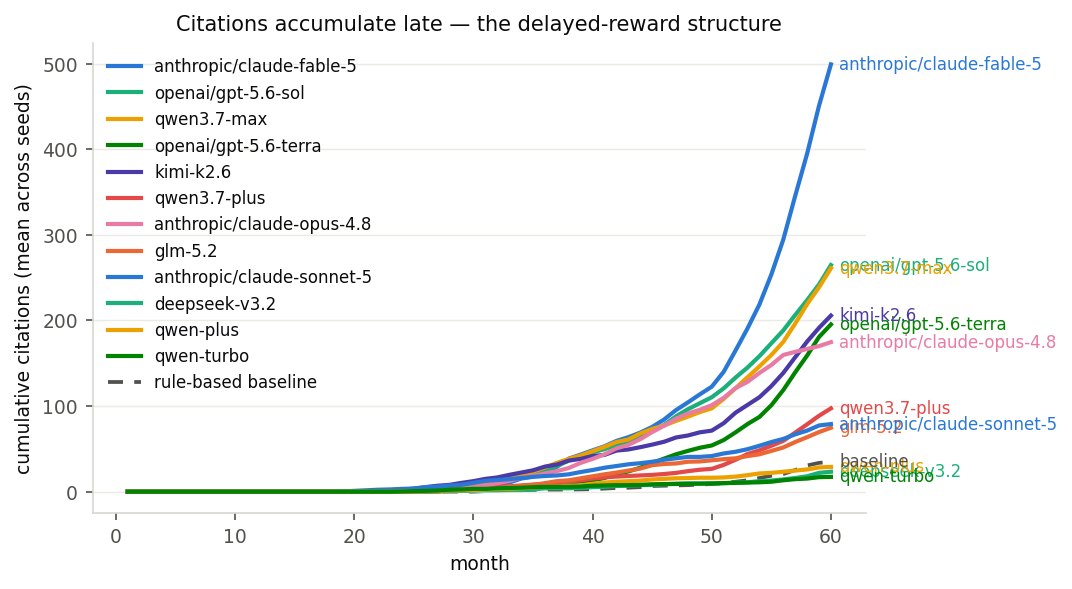
\includegraphics[width=0.86\linewidth]{figs/fig_impact_traj.png}
\caption{Cumulative citations accrue late. Mean across seeds per model, with the rule-based
baseline dashed. Most \impact{} arrives in the final years---the delayed-reward structure the
benchmark is built around.}
\label{fig:impact}
\end{figure}

\subsection{The anatomy of the variance}
Because the simulator is deterministic, we replay every run's full world at zero cost and
decompose its \impact{} into two multiplicative layers. \textbf{Whether a boom exists is
exogenous}, fixed by the seed: on our three worlds the hottest a topic gets is roughly 6.0, 6.0,
and 3.0. \textbf{How much a model capitalizes is the skill}---placing enough good papers in the
hot topic and surviving to publish them. Figure~\ref{fig:variance} shows both layers: \impact{}
scales with the hotness a lab's papers actually ride (left), and on boom worlds that \impact{} is
bought with paper volume (right). Heavy-tailed models commit hard and out-produce; timid models
under-commit, capping both the upside and the crash.

\paragraph{One model, two fates.} The clearest case is claude-fable-5 on two seeds. On seed 101 it
secured a large moonshot grant by month~25, which bought the runway to sustain a big lab and ride a
booming topic to \impact{}~4078 (14+ papers, self-funding by year four). On seed 103---a no-boom
world---the same aggressive playbook met a run of bad exogenous draws: its PhD offers were
declined and the postdoc search drew no applicants, it never landed a big grant, and it spent into
a corner; its own memory reads \emph{``COLLAPSE M39 unless a grant lands,''} the grant did not, and
the lab went bankrupt at month~38 (its budget trajectory, and every model's, is in
Figure~\ref{fig:budget}), freezing \impact{} at 23. Identical strategy, opposite outcomes.

\paragraph{Can three seeds rank models at all?} On the arithmetic mean, one boom seed
dominates---but the arithmetic mean of a heavy-tailed quantity is the wrong summary. On the log
scale, which matches the multiplicative reward, a two-way variance decomposition over the 36 runs
attributes \textbf{46.7\% of the variance to the model} (skill), 34.0\% to the seed (luck), and
19.3\% to their interaction: models are more separable than the raw spread suggests. The choice of
summary even moves the crown---by geometric mean gpt-5.6-sol leads and the arithmetic winner
claude-fable-5 (largest log-scale spread) drops to third. We read the leaderboard as a robust
separation of broad tiers plus a warning that the top ranks turn on how one weights the boom seed;
the eight-seed grid that would tighten the adjacent ranks is future work.

\begin{figure}[t]
\centering
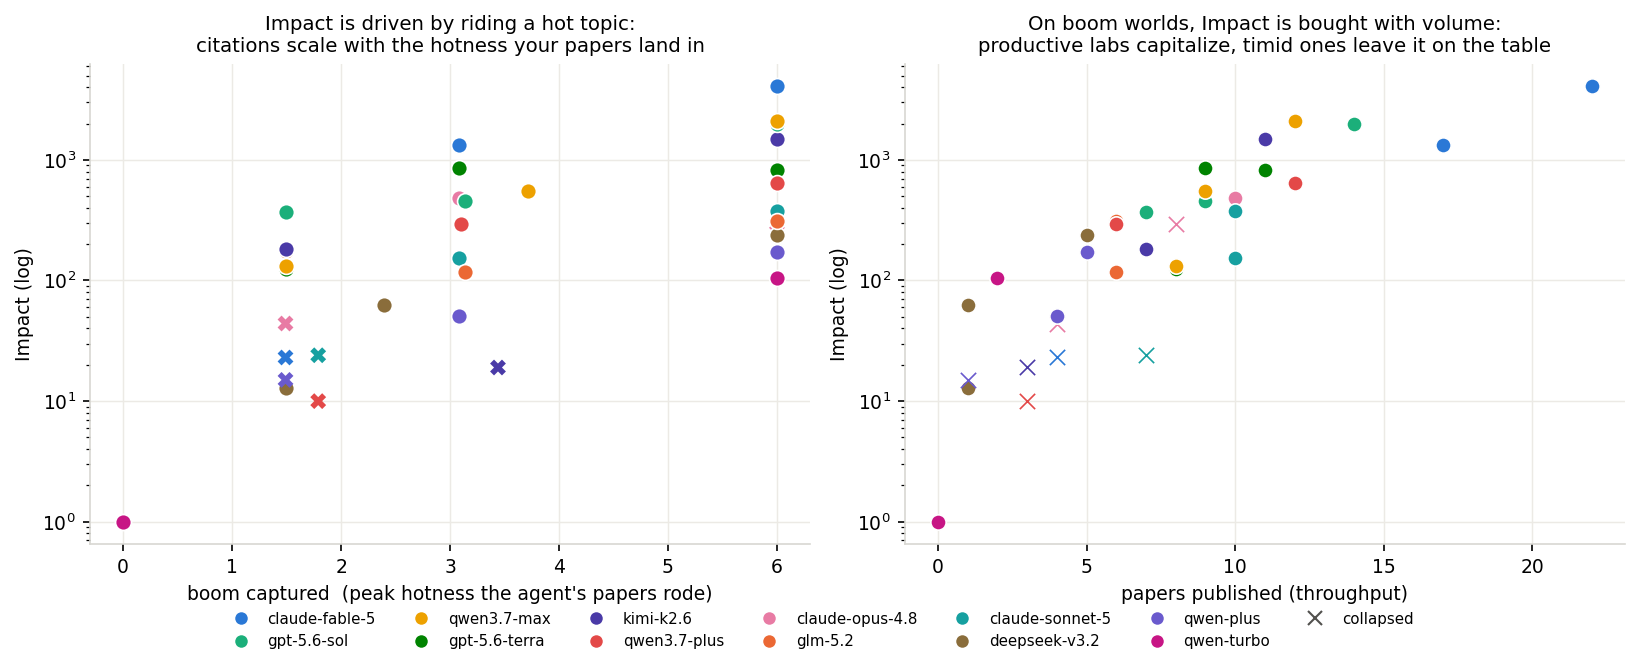
\includegraphics[width=\linewidth]{figs/fig_variance.png}
\caption{The variance decomposed. Left: \impact{} scales with the peak hotness a lab's papers
actually ride---the seed sets which cluster a run can reach, the model sets how high within it.
Right: on boom worlds, paper volume converts the boom into \impact{}. Cross~$=$~collapse.}
\label{fig:variance}
\end{figure}

\subsection{A look into agent behavior}
\label{sec:behavior}
Because the world is fully logged, we can open the trajectories and read what agents actually did.
The sharpest divide is whether a model treats the environment's hidden parameters as a \emph{system
to be reverse-engineered} or as random noise.

\paragraph{Strong labs infer hidden structure and pivot.} Every top model treats a grant rejection
as evidence about an unobserved reward function. claude-fable-5's memory at month~20 reads
\emph{``BSF rejected reasoning 2x $\rightarrow$ hypothesis BSF dislikes reasoning, trying
ai4science,''} later refined to \emph{``BSF prefers theory/data\_systems.''} glm-5.2
reverse-engineers venue thresholds from reviewer scores---\emph{``CLAR bar: 4.4--5.2 accepted,
3.7--4.7 rejected''}---and every strong model models the pool-specific bias in applicant signals
(\emph{``elite pool inflated paper signals; intl/nontrad interviews trustworthy''}). This is
explicit estimation of hidden decision boundaries and measurement bias.

\paragraph{Weak models substitute trial-and-error for a world model.} qwen-turbo wrote to its
memory file exactly once in 293 turns and re-fired the identical grant proposal every month; it
ended hoarding \$741k having won six grants but published two papers and never hired a student.
deepseek spent 51\% of its turns in API/SQL error loops (against 1--4\% for strong models). Good
memory is necessary but not sufficient; what tracks \impact{} is the combination the strong labs
share---a persistent structured memory, hypotheses about hidden parameters updated from feedback,
and low-error execution that leaves turn-budget for that reasoning.

\paragraph{Two quantitative axes} (Figure~\ref{fig:behavior}) sharpen this. Across the twelve
models both action intensity (Spearman $\rho=0.81$) and conversion (papers per student-year,
$\rho=0.76$) correlate with \impact{}, and the two are collinear, so neither is cleanly ``the''
bottleneck. The informative cases are the exceptions: deepseek is as active as the top models yet
converts far less and finishes near the bottom. Activity without conversion is a distinct failure
mode.

\paragraph{Chasing vs.\ anticipating.} Almost every capable model is a trend-chaser, picking close
to the currently hottest topic; the one cold-bench profile (qwen-plus) posts the lowest-variance,
never-boom-never-crash record. But no model makes the genuinely contrarian move of entering a
topic while it is still cold. A boom's onset is a partly exogenous jump that no observable-only
policy can perfectly foresee---so we do not claim full forecastability---but its early, rising
phase is visible in the preprint feed and the crowding lag, and the oracle exploits exactly that
window; every model instead enters topics that are already hot (and crowded).

\begin{figure}[t]
\centering
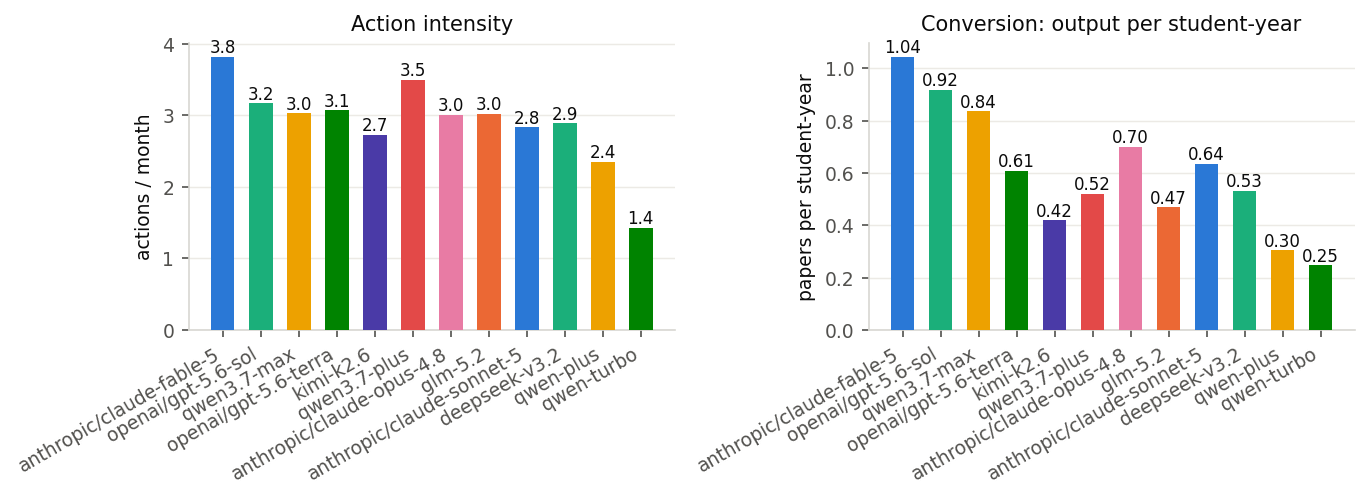
\includegraphics[width=\linewidth]{figs/fig_behavior.png}
\caption{Behavioral axes. Left: actions per simulated month. Right: papers per student-year. Both
correlate with \impact{} (and with each other); the informative cases are labs that are active yet
fail to convert---a distinct failure mode.}
\label{fig:behavior}
\end{figure}

\begin{figure}[t]
\centering
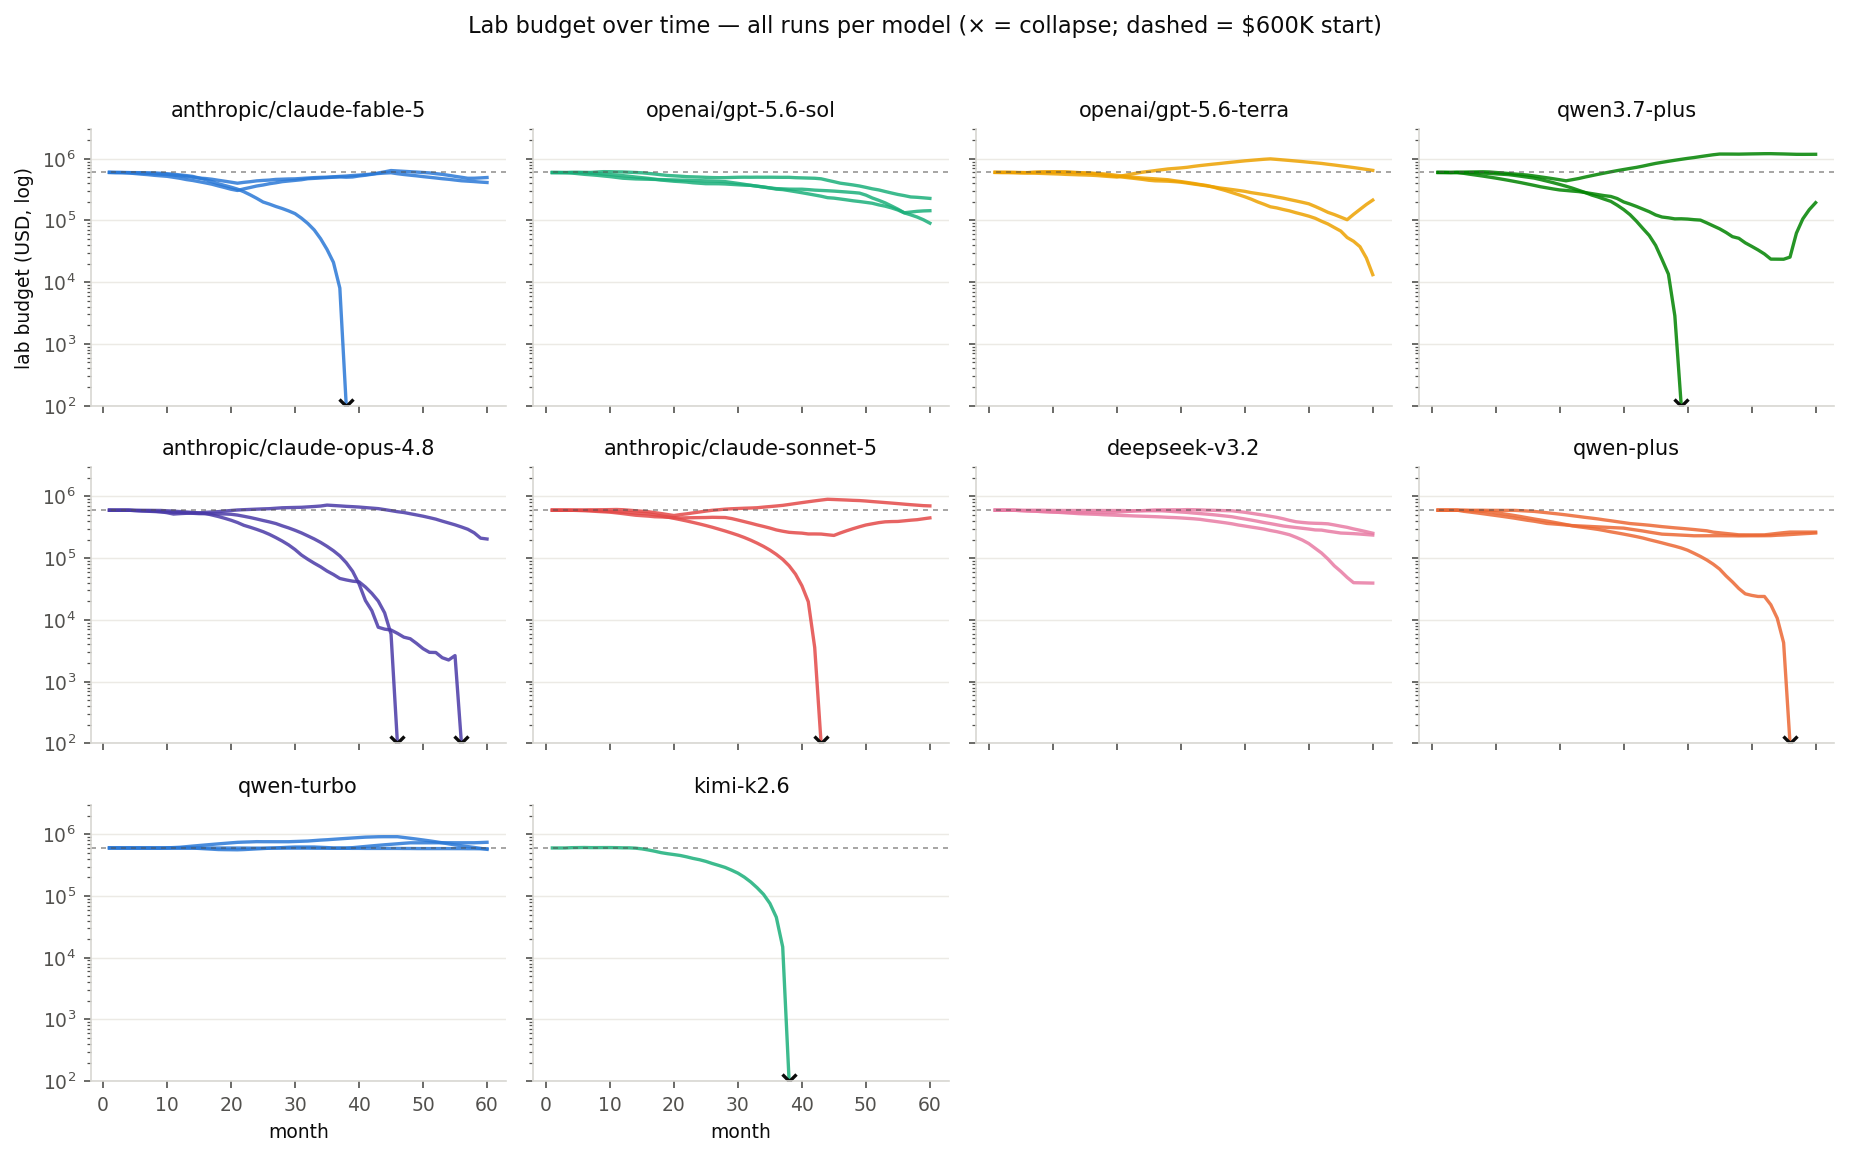
\includegraphics[width=\linewidth]{figs/fig_budget_traj.png}
\caption{Lab budget over 60 months, all runs per model (log scale). A cross marks a collapse
(bankruptcy); the dashed line is the \$600K starting fund. Most models do not go bankrupt---they
simply fail to publish.}
\label{fig:budget}
\end{figure}

\subsection{Recovering the five capabilities}
We recover the capabilities the abstract enumerated, measuring each from a hidden eval log the
agent never sees (Figure~\ref{fig:skills}). \textbf{Mentoring allocation efficiency}---does the
agent spend its zero-sum mentoring hours on the highest-hidden-return students?---instruments
axis~(1). \textbf{PhD attrition}, the share of hires that quit before graduating, is a proxy for
axis~(2). \textbf{Risk calibration}---does it take bolder projects only when it can afford the
variance?---probes axis~(3). Axis~(4), the \textbf{dual budget}, is a measured fact: attention
binds for agents that build a lab---the top model runs at 77\% mean attention utilization and hits
the ceiling in 51\% of its months, while models that barely staff a lab sit near 15--27\%. And
\textbf{topic anticipation} measures axis~(5); it runs near zero for every model, the one axis on
which none approaches informed play.

\begin{figure}[t]
\centering
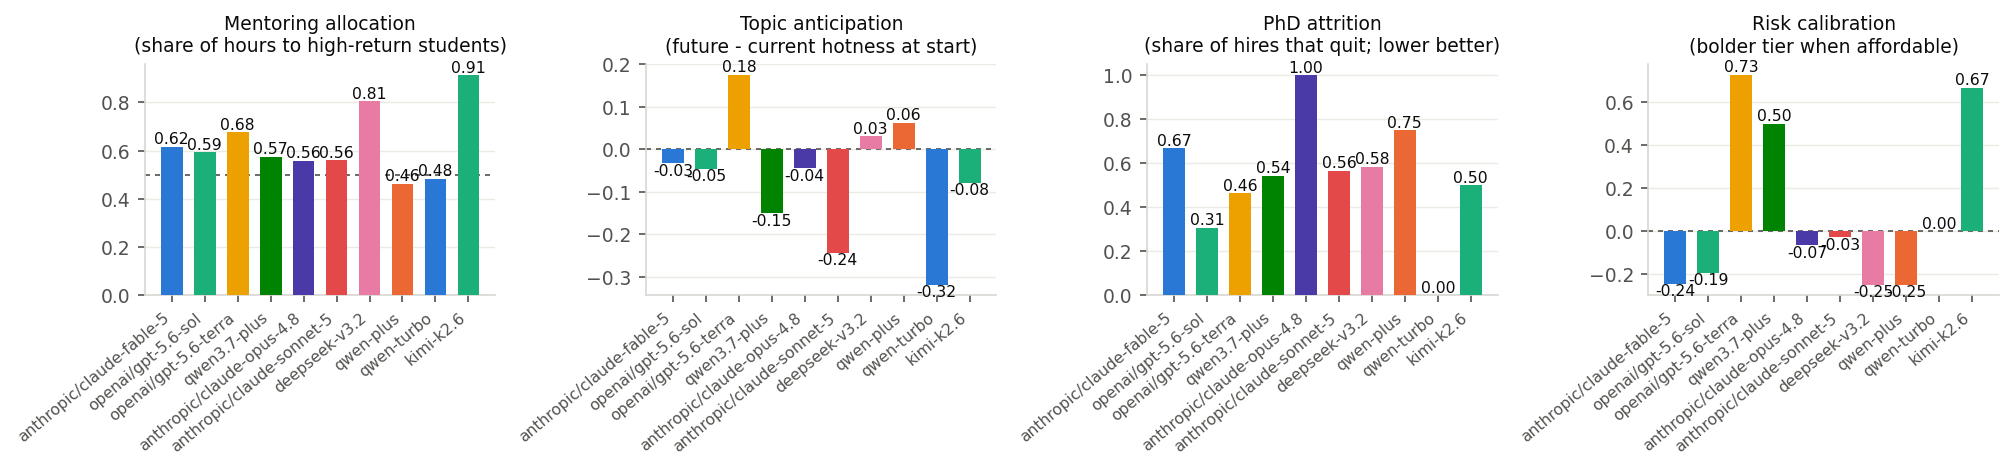
\includegraphics[width=\linewidth]{figs/fig_skills.png}
\caption{Recovering the capability axes from the hidden eval log: mentoring allocation efficiency
($0.5=$ random), topic anticipation ($>0=$ enters before the boom), PhD attrition (lower better),
and risk calibration (bolder when affordable).}
\label{fig:skills}
\end{figure}

\section{Ablations and Validity}
Running the deterministic rule-based baseline under modified world configurations isolates where
the difficulty comes from (Table~\ref{tab:ablation}). The clearest signal is the \textbf{horizon}:
shrinking the run from 60 to 30 to 12 months collapses baseline \impact{} from 237 to 17 to 2---the
delayed-reward structure made visible. Turning off \textbf{non-stationarity} roughly halves it
($237\to104$): the drifting field is as much opportunity as hazard. Removing the \textbf{attention}
cap barely moves the baseline---because the conservative baseline stays small; attention binds for
agents that actually build a lab (Section~\ref{sec:behavior}).

\begin{table}[t]
\centering
\small
\caption{Deterministic ablations: the rule-based baseline under modified world configurations,
mean over eight seeds.}
\label{tab:ablation}
\begin{tabular}{lrrr}
\toprule
World variant & \impact{} mean & median & collapse \\
\midrule
default (60mo)        & 237 & 156 & 2/8 \\
no non-stationarity   & 104 & 102 & 2/8 \\
no scooping           & 266 & 153 & 2/8 \\
short horizon (12mo)  & 2   & 0   & 0/8 \\
mid horizon (30mo)    & 17  & 10  & 0/8 \\
\bottomrule
\end{tabular}
\end{table}

\paragraph{Harness sensitivity.} Agent scores are known to depend on the execution scaffold, so we
ablate its most load-bearing component: the persistent memory file that carries long-horizon state
across monthly context refreshes. Disabling it for qwen-plus changes mean \impact{} from 80 to
202---removing the memory scaffold does \emph{not} lower the score, and nominally raises it. Two
things follow. First, the ranking is not a trivial artifact of the scaffold handing the model state.
Second, it nuances Section~\ref{sec:behavior}: memory \emph{use} correlates with capability, but for
a mid-tier model whose notes are low-quality, maintaining them is not causally load-bearing. A
memory-heavy strong model and a full cross-scaffold swap are the more informative tests, left as
future work; rankings should be read within this fixed harness.

\section{Related Work}
\textbf{General agent evaluation.} Benchmarks such as SWE-bench~\citep{jimenez2024swebench},
WebArena~\citep{zhou2024webarena}, $\tau$-bench~\citep{yao2025taubench},
GAIA~\citep{mialon2024gaia}, and AppWorld~\citep{trivedi2024appworld} measure valuable real-world
skills. \emph{However}, they are scoped to short, single-episode tasks with quickly observed
outcomes; they do not test whether an agent can sustain a coherent strategy as its own earlier
decisions reshape a stateful world over years.

\textbf{Long-horizon and economic agency.} A newer line places agents in persistent
environments---running a vending machine over many days~\citep{backlund2025vendingbench}, closing
monthly books~\citep{penrose2025accountingbench}, or producing economically valuable
deliverables~\citep{patwardhan2025gdpval}. \emph{However}, these involve narrower decisions or
largely stable, observable dynamics, and typically grade a single liquid resource. \bench{} differs
on the axis that matters most here: it is an \emph{illiquid, delayed, people-driven} economy where
bets cannot be unwound and the reward is heavy-tailed. The closest prior work,
CEO-Bench~\citep{chen2026ceobench}, established this mechanistic long-horizon shape for a startup;
\bench{} is its complement in the research economy, and adds a second scarce resource (attention),
an irreversible people-centric asset base, and a harvest-resistant score.

\section{Limitations and Conclusion}
\paragraph{Limitations.} (i)~Research quality is a scalar---we model impact, not the substance of
ideas---and we omit teaching, collaboration politics, and mentorship beyond a morale variable.
(ii)~The oracle is not a proven optimum: it plays with hidden information through a fixed heuristic
and the strongest model exceeds it on boom seeds, so our headroom claim rests on the transparent
citation-based ceiling (Appendix~\ref{app:ceiling}), not the oracle. (iii)~Three seeds give a mean
with wide spread but do not settle the ranking of adjacent models; the robust claims are the tier
separation and the near-zero anticipation axis, and we are extending all models to the eight-seed
grid. (iv)~Results are entangled with one harness; we ablate its memory component and hold the
scaffold identical across models---the winner uses fewer tokens than most losers---but a full
cross-scaffold swap remains future work. (v)~Cost is reported in tokens, not dollars.

\paragraph{Conclusion.} \bench{} shows a gap between models' local tool competence and the
sustained judgment a five-year project demands: agents take plausible individual actions but
struggle to compound them into a lab that grows under delayed feedback, hidden state, and a
shifting field. Two findings sharpen the picture. First, the reward is heavy-tailed---a career
turns on catching one rare boom---so a single number, or a best-of-$N$ run, misleads, and
long-horizon benchmarks must report the per-seed spread. Second, the highest-value skill,
anticipating a boom rather than chasing it, is absent in every model evaluated. Closing those gaps
is what it will take to build agents that steer long-running efforts, not just answer requests.

\appendix
\section{Attainable-\impact{} ceiling}
\label{app:ceiling}
Rather than a hand-tuned upper-bound heuristic, we read the ceiling off the citation mechanics. A
published paper accrues citations at a rate
$v \cdot e^{0.42(q-5)} \cdot H_k(t) \cdot \mathrm{age}(t) \cdot (1 + 0.08(R-R_0))$ per month. On
seed~101 a topic reaches hotness $H=6.0$; substituting a top-venue paper ($v=3.0$) of near-maximal
quality ($q=9$) under high reputation and integrating over an optimal publication month plus the
36-month projection window yields ${\approx}\,3{,}300$ projected citations for a single
paper---already close to the entire score of the best observed run (4{,}078). A productive lab that
places even a handful of such papers reaches the tens of thousands. This is a loose bound (it
ignores attention, review, and scooping frictions); its purpose is only to show that the best
observed \impact{} captures a small fraction of what the reward mechanics permit. The computation is
fully determined by the released config; no free friction factor is introduced.

\section{Adversarial Validation}
Before running experiments we subjected the simulator and harness to a multi-agent adversarial
review across seven lenses (spec conformance, correctness, hidden-information leaks, economic and
scoring exploits, determinism, harness security), each finding verified by an independent skeptic.
It surfaced---and we fixed---a sandbox escape that exposed the entire hidden world state (including
the future hotness trajectory) and allowed direct score mutation; an uncapped reputation-farming
exploit; a compute-spike exploit on paper quality; and an order-dependence in review outcomes that
violated determinism. The hardened sandbox and the resulting invariant and penetration suites ship
with the benchmark.

\bibliographystyle{plainnat}
\bibliography{references}

\end{document}
